

\chapter{The Net Carbon Impact of this PhD}\label{ch:impact}

In this short concluding Chapter, I will estimate the \ch{CO2} emitted and (Section \ref{sec:burning}), with much more uncertainty, the expectation value of the \ch{CO2} saved during my PhD project (Section \ref{sec:millivolt}). The idea is to determine whether I have done any net good during the past three years with respect to the climate crisis described in Chapter 1.

A version of this question, rearranged to be a bit more rigorous, is:
\begin{question}
	What portion of a millivolt's improvement in efficiency of PEM electrolyzers worldwide in the year 2030 would have to be attributable to my research in order to offset the \ch{CO2} footprint of my PhD project? \label{q:impact}
\end{question}

Finally, the last Section will serve as a conclusion and outlook for this Thesis.


\section{Burning}



\section{How much difference a millivolt makes}

Answering Question \ref{q:impact} requires an estimate of how much hydrogen is produced by PEM electrolyzers in 2030, and some assumptions of how it is used.

These estimates are the job of \textit{energy systems modeling}, which involves minimizing costs for an energy system given technoeconomic parameters of the technologies and resources available, and subject to constraints such as a cap on \ch{CO2} emissions\cite{Storgaard2019_MSc}. Results of the models vary a lot, depending on the region modeled, the assumptions made, and the techniques used. Almost all predict a role of hydrogen from water electrolysis in the energy system starting around 2030, but the amount varies a lot, with predictions of anything from 2\% to 8\% of total electricity generation going to hydrogen production in 2030. The usage of hydrogen also varies, from primarily energy storage\cite{Budischak2013, Storgaard2019_MSc, Jacobson2018} to primarily fuel cell electric vehicles\cite{Meibom2010} to primarily decarbonization of industry by steel production \cite{Sgobbi2016}. 

To estimate the impact of a marginal improvement in electrolyzer efficiency, I make the following assumptions:

\begin{itemize}
	\item 2\% of European electricity generation goes to \ch{H2} production by water electrolysis\cite{Sgobbi2016} (that study assumes alkaline electrolyzers, but PEMEC's are widely believed to be the dominant technology in 2030 \cite{Schmidt2017}).
	
	\item The electrolyzer cells run at a cell potential 1.7 V, representative of those compared in ref. \citen{Sgobbi2016}.
	
	\item The amount of power going to hydrogen is constant, such that the improvement in efficiency results in more \ch{H2}.
	
	\item The extra \ch{H2} is used to generate electricity with a round-trip efficiency of 46\%, the value used in ref. \citen{Sgobbi2016}.
	
	\item The extra \ch{H2} displaces fuels which would have generated electricity at a carbon intensity of 340 kg/MWh, which is the average for European electricity today\cite{Moro2018}. This also represents some uncertainty. If the \ch{H2} replaces coke in steel production, the savings are greater. If it replaces bio-fuel from a plant fitted with carbon capture and storage, the savings might be less.
	
	\item \ch{CO2} costs associated with implementing the hypothetical improvement in PEMEC's or storing the extra hydrogen are negligible
\end{itemize}
Finally, the big assumption - the one that has to do with my work. 
\begin{itemize}
	\item My research will result in an improvement in electrolyzer efficiency of 0.05 mV for a period of 1 year. 
\end{itemize}
This should be considered an expectation value. Maybe the research in this PhD project never leads to any change, but maybe it leads to a much bigger change than expected. This could be interpreted as a 1\% chance of a breakthrough that improves PEMEC's by 5 mV. Or one twentieth of the work that is needed to make a more modest breakthrough worth 1 mV. Or perhaps, though unlikely, the methods developed here are a step towards rational design of a reversible acid-stable OER catalyst saving 200 mV. There is no way to know as of yet. The use of one twentieth of a milivolt as an expectation value feels modest and reasonable, but I must admit that it is completely arbitrary. The period of one year is also arbitrary, but a finite time period over which the impact applies is necessary for the calculation. It could be taken to represent the fact that someone else, by other means, would have likely made the same progress shortly after, so my PhD project might at best be speeding things up. Because of these arbitrarinesses, in a bit, therefore, I will take out this assumption and instead look at through the window of Question \ref{q:impact}, i.e. how big would the impact \textit{have to be} for my PhD project to break even in the climate account.

To calculate the \ch{CO2} saved, then, the first step is to calculate the amount of extra hydrogen generated. The amount of hydrogen generated (in mols) without the improvement is
\begin{equation}
n^{\ch{H2}}_0 = 2\mathcal{F} \frac{xP_0}{V_\text{EC}}\,,
\end{equation}
where $\mathcal{F}$ is Faraday's constant, $x$ is the portion of total electricity generated which goes to hydrogen production, $V_\text{EC}=1.7$ V is the electrolyzer potential without the improvement, and $P_0$ is the total amount of electricity generated. For the EU in 2018, $P_0=3.1\cdot10^9$ MWh. The quantity $xP_0/V_\text{EC}$ is the total amount of charge going to hydrogen generation during the period.

With an improvement (decrease in cell potential) of $\Delta V$, the amount of hydrogen generated is
\begin{equation}
n_1 = \frac{1}{2\mathcal{F}} \frac{xP_0}{V_\text{EC}-\Delta V}\,.
\end{equation}
The difference is
\begin{equation}
\Delta n = n_1 - n_0 = \frac{xP_0}{2\mathcal{F}}\left(\frac{\Delta V}{V_\text{EC}(V_\text{EC}-\Delta  V)}\right) \approx \frac{xP_0\Delta V}{2\mathcal{F} V_\text{EC}^2}\,,
\end{equation}
where the last step has used the fact that it is only a marginal improvement, i.e. $\Delta V \ll V_\text{EC}$.

When this hydrogen is fed back into the electricity system through a fuel cell, the amount of electricity it generates is
\begin{equation}
\Delta P = 2\mathcal{F} \Delta n V_\text{FC} = xP_0 \frac{V_\text{FC}\Delta V}{V_\text{EC}^2} = xP_0\eta \frac{\Delta V}{V_\text{EC}}\,,
\end{equation}
where $V_\text{FC}$ is the voltage of the fuel cell and $\eta = V_\text{FC}/V_\text{EC}$ is the round-trip efficiency. The \ch{CO2} saved is then
\begin{equation}
s = \sigma x P_0 \eta \frac{\Delta V}{V_\text{EC}}\,,\label{eq:savings}
\end{equation}
Where $\sigma$ is the carbon intensity of the fuel that hydrogen is replacing to generate $\Delta P$ of electricity.
\begin{figure}[h!]
	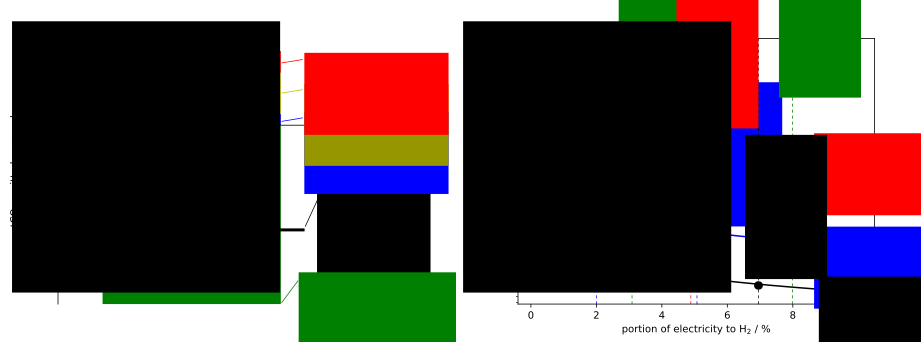
\includegraphics[width=1\textwidth]{05_Impact/fig/net_impact.png}
	\caption{\textbf{(a)}, \ch{CO2} emissions (red, yellow, and red) and savings (green) associated with this PhD project with the assumptions described in the Figure and in the text. \textbf{(b)} Millivolts of improvement in electrolyzer operating potential needed to offset the \ch{CO2} emissions of this PhD project in one year as a function of the percentage of the electricity generated in Denmark (red), Europe (blue), or the world (black) that goes to \ch{H2} production. Several predicted \ch{H2} penetrations from literature are included with their area of study indicated: [A], Sgobbi et al, 2016, ref. \citen{Sgobbi2016}; [B], Budischak et al, 2013, ref. \citen{Budischak2013}; [C], Meibom and Karlsson, 2010, ref. \citen{Meibom2010}; [D], Jacobson et al, 2018, ref. \citen{Jacobson2018}; [E] Storgaard, 2019, ref. \citen{Storgaard2019_MSc}}
	\label{fig:impact}
\end{figure}

Plugging in the numbers from the assumptions above, the expectation value of the \ch{CO2} emissions saved by this PhD project is
\begin{equation}
s = 340 \left[\frac{\text{kg}_{\ch{CO2}}}{\text{MWh}}\right] \cdot 2 [\%] \cdot 3.1\!\cdot\! 10^9 \text{[MWh]} \cdot 46 [\%] \cdot \frac{0.05 \text{[mV]}}{1.7 \text{[V]}} = 293 \,[\text{t}_{\ch{CO2}}]
\end{equation}
This is very good news, because it is greater than the 122 tons of \ch{CO2} emissions that I estimated to result from this PhD project! This is illustrated in Figure \ref{fig:impact}a.

The problem is turned around in Figure \ref{fig:impact}b. Here, I am inquiring into the break-even point. I have set the savings $s$ from Equation \ref{eq:savings} equal to the costs $c$ from Equation \ref{eq:costs} and solved for $\Delta V$:
\begin{equation}
\Delta V = \frac{c V_\text{EC}}{\sigma x P_0 \eta}
\end{equation}
The solution is plotted as $\Delta V$ vs $x$ for three values of $P_0$ corresponding to the total electricity generated in 2018 for Denmark \cite{EnergiNet}, Europe \cite{EEA2018}, and the world \cite{Enerdata2019}.

Clearly, scale matters. If improvements resulting from this PhD project stay in Denmark and the portion of electricity used for hydrogen generation doesn't exceed 5\%, then my work needs to be worth a millivolt by itself to pay for its \ch{CO2} cost in a year. On the other hand, if the hypothetical improvement spreads to the whole world and the portion of electricity used for hydrogen generation globally does exceed 5\%, then a contribution worth as little as a microvolt will do the trick.

\label{sec:millivolt}



\section{Conclusion}\label{sec:conclusion}